\documentclass[a4paper,11pt]{article}
\usepackage{lecturenotes}
\usepackage{amsmath}
\lectureheader{ELE745}{1}
\begin{document}
\tableofcontents
\clearpage
\notesection{Overview of Digital Communication Systems}
\begin{figure}[htbp]
    \centering
    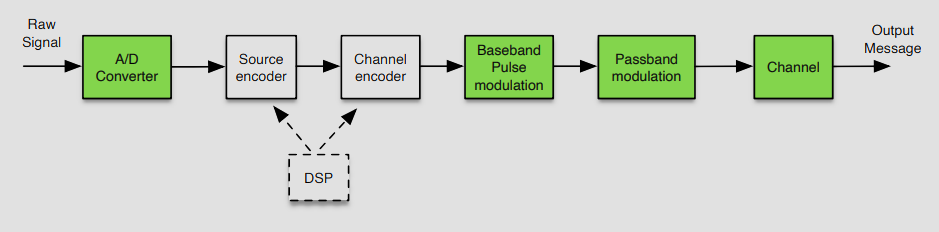
\includegraphics[width=0.8\linewidth]{figures/digital-communication-system-flow.png}
    \caption{Digital Communication System}
    \label{Digital-Comm-Sys}
\end{figure}
\begin{notetable}{l X}{\textbf{Component} & \textbf{Definition}}
    Source Encoder & Remove redundancy existing in source transmission so \# of bits required to represent signal is smaller \\
    Channel Encoder & Introduce controlled redundancy to info bits to combat channel loss \\
    Baseband Modulation & Generate waveform suitable for tranmission \textit{- covert digital back to analog} \\
    Passband Modulation & Translate baseband waveform $g_i(t)$ to a frequency that is greater than the spectral contents of $g_i(t)$ via carrier wave \\
    Channel Bandwidth, $\mathbf{B_C}$ & The range of frequencies that it can transmit with reasonable fidelity \\
    Signal Bandwidth, $\mathbf{B_M}$ & The highest frequency component inside a signal \\
\end{notetable}

\notedefinition{Successful Tranmission}{$B_C \geq B_M$}

\notesection{Channel Capacity}
\keyequation{Shannon Equation of AWGN Channel}{C = B_c log_2 (1+ SNR) \qquad \text{bits/s}}[
    Where:
    \begin{itemize}
        \item $B_C$ limits the signal bandwidth that can succesfully pass through
        \item SNR at the reciever determines the recoverabiltiy of the transmitted signal
        \item C is the upper bound on the rate of information transmitted per second
    \end{itemize}
]
\notedefinition{Channel  Capacity}{Peak throughput that can be realiably carried by a channel}

\notesection{Overview of Signals and Systems}
\subnotesection{Signal Power and Energy}
A energy signal has finite amount of total normalized energy over all time. Meanwhile, a power signal continues indefinitely and has a finite, non-zero average power.
\keyequation{Signal Energy}{E_g = \int_{-\infty}^{\infty} g^2(t) dt = \int_{-\infty}^{\infty} |g(t)|^2dt}
There are a large class of signals for which $E_G$ is not finite, for these signals we can use signal power equations.\newline
\keyequation{Signal Power}{P_G = \lim_{t \rightarrow \infty} \frac{1}{T} \int_{-\frac{T}{2}}^{\frac{T}{2}}|g(t)|^2 dt}
\textbf{Signal Power}

Both $E_G$ and $P_G$ do not indicate true energy or power. If g(t) is a voltage waveform, then $E_G$ and $P_G$ represent unit energy/power delivered across 1 $\Omega$ resistor.
Observe that $|g(t)|^2 = g(t) g^{*}(t)$ where the * denotes the complex conjugate. The standard units of signal energy and power are the \text{joule (J)} and \text{watt (W)} respectively. A logarithimic scale is used, therefore a signal with average power P watts has power of:

\keyequation{Average Power}{P_{avg} = [10 \cdot log_10 P] \quad \text{or} \quad [30 + 10 \cdot log_10 P] dBm}

The \textbf{RMS value} of a signals average power can be found by taking the square root of the average power. Therefore, the RMS value of a signal with average power $P_{avg}$ is:
$$
    P_{RMS} = \sqrt{P_{avg}}
$$

\notesection{Classification of Signals}

A \textbf{Deterministic Signal} is a signal that has no uncertainty w.r.t its value at any time. While a \textbf{Random Signal} has uncertainty, where its value is determined by its statistical properties. \\
Some other keywords related to signal properties that are obvious:
\begin{itemize}
    \item \textbf{Continuous time} and \textbf{discrete time} signals
    \item \textbf{Periodic} signals and \textbf{non-periodic} signals
    \item a \textbf{analog} signal has any value in a continuous range
    \item a \textbf{discrete} signal has an amplitude which can only take on a finite number of values
\end{itemize}

\notesection{Useful Signal Operations}

\begin{notetable}{l X}{\textbf{Operation Name} & \textbf{Operation}}
    Time-shift & $g(t) \rightarrow g(t-t_0)$ \\
    Time-reversal & $g(t) \rightarrow g(-t)$ \\
    Time-scale & $g(t) \rightarrow g(at)$ \\
\end{notetable}

Note for a time-scale operation: if $a>1$, the scaling is \textbf{compression}, and if $a<1$, the scaling is \textbf{expansion}
\begin{figure}[htbp]
    \centering
    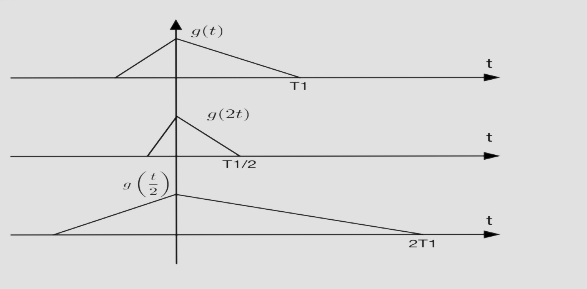
\includegraphics[width=0.8\linewidth]{figures/time-scaling-operation.png}
    \caption{Time-scaling Operation}
    \label{Time-scaling-op}
\end{figure}

\notesection{Important Functions}
\subnotesection{Unit Impulse}
\begin{tikzpicture}[x=1.4cm,y=1.4cm]

    % Time axis
    \draw[->] (-2.5,0) -- (2.5,0) node[right] {$t$};

    % Origin
    \node[below left] at (0,0) {$0$};

    % Unit impulse
    \draw[->,very thick] (0,0) -- (0,1.5);
    % Weighted and Shifted
    \draw[->,very thick] (1.5,0) -- (1.5,1.5);
    \node[left] at (1.5,1.5) {$A$};
    \node[above right] at (1.5,1.5) {$A\delta(t-t_0)$};
    % Labels
    \node[left] at (0,1.5) {$1$};
    \node[above right] at (0,1.5) {$\delta(t)$};
\end{tikzpicture}

The following properties are important to this function:
\begin{align*}
     & \delta(t) = 0 \quad \text{when} \quad t \neq 0 \\
     & \int_{-\infty}^{\infty} \delta(t) dt = 1
\end{align*}

Multiplying a unit impulse function by a function, $\phi (t)$ we get:
$$
    \phi(t)\delta(t-T) = \phi(T)\delta(t-T)
$$
Similarly, the sampling property of the unit impulse function is:
$$
    \int_{-\infty}^{\infty} \phi(t) \delta(t-T)dt = \phi(T) \int_{-\infty}^{\infty} \delta(t-T)dt = \phi(T)
$$
\subnotesection{Unit Sinc Function}
The \textbf{sinc} function is defined as: $Sinc(x) = \frac{sin(x)}{x}$, some of its properties include:
\begin{itemize}
    \item Sinc(x) is an even function of x
    \item Sinc(x) = 0 when sin(x) = 0 expect at x = 0, where it is determined. Therefore: $sinc(x) = 0 \quad \text{for} \quad x = \pm n \pi$
    \item When evaluating the value at t = 0 we use: $$\lim_{x \rightarrow 0} sinc(x) = \lim_{x \rightarrow 0} \frac{sin(x)}{x} = \lim_{x \rightarrow 0} \frac{cos(x)}{1} = 1$$
\end{itemize}
\notedefinition{Sinc(x) Summary}{An even oscillating function with decreasing amplitude. It has a unit peak at x = 0, and a zero crossing at integer multiples of $\pi$}
\subnotesection{Other Important Functions}
\begin{tcbraster}[raster columns=2, raster equal height=rows,
        raster column skip=6pt, raster row skip=6pt,
        colback=white, colframe=NoteRule, boxrule=0.6pt, arc=2pt,
        left=8pt, right=8pt, top=8pt, bottom=8pt]
    \begin{tcolorbox}
        {\sffamily\bfseries\color{NoteAccent}Unit Comb}\par
        \begin{minipage}[c][2.8cm][c]{\linewidth}
            \centering
            \begin{tikzpicture}[x=0.72cm,y=0.75cm]
                \draw[->] (-3.6,0) -- (3.7,0) node[right] {\scriptsize $t$};
                \foreach \k in {-3,-2,-1,0,1,2,3}{
                        \draw[->,thick,NoteAccent] (\k,0) -- (\k,1);
                    }
                \node[below,font=\scriptsize] at (-2,0) {$-2T$};
                \node[below,font=\scriptsize] at (-1,0) {$-T$};
                \node[below,font=\scriptsize] at (0,0) {$0$};
                \node[below,font=\scriptsize] at (1,0) {$T$};
                \node[below,font=\scriptsize] at (2,0) {$2T$};
                \node[left,font=\scriptsize] at (-3,1) {$1$};
                \node at (-3.45,0.6) {$\cdots$};
                \node at (3.45,0.6) {$\cdots$};
            \end{tikzpicture}
        \end{minipage}\par
        {\small\centering
            $\displaystyle \operatorname{comb}_T(t)
                = \sum_{n=-\infty}^{\infty}\delta(t-nT)$\par}
    \end{tcolorbox}%
    \begin{tcolorbox}
        {\sffamily\bfseries\color{NoteAccent}Unit Rectangle}\par
        \begin{minipage}[c][2.8cm][c]{\linewidth}
            \centering
            \begin{tikzpicture}[x=1.65cm,y=1.15cm]
                \draw[->] (-1.6,0) -- (1.7,0) node[right] {\scriptsize $t$};
                \draw[->] (0,-0.3) -- (0,1.4);
                \draw[very thick,NoteAccent] (-1.4,0) -- (-0.5,0)
                (-0.5,0) -- (-0.5,1) -- (0.5,1) -- (0.5,0)
                (0.5,0) -- (1.4,0);
                \node[below,font=\scriptsize] at (-0.5,0) {$-\frac12$};
                \node[below left,font=\scriptsize] at (0,0) {$0$};
                \node[below,font=\scriptsize] at (0.5,0) {$\frac12$};
                \node[left,font=\scriptsize] at (0,1) {$1$};
            \end{tikzpicture}
        \end{minipage}\par
        {\small\centering
            $\displaystyle \operatorname{rect}(t)=
                \begin{cases}
                    1,       & |t|<\frac12, \\
                    \frac12, & |t|=\frac12, \\
                    0,       & |t|>\frac12.
                \end{cases}$\par}
    \end{tcolorbox}%
    \begin{tcolorbox}
        {\sffamily\bfseries\color{NoteAccent}Unit Step}\par
        \begin{minipage}[c][2.8cm][c]{\linewidth}
            \centering
            \begin{tikzpicture}[x=1.15cm,y=1.15cm]
                \draw[->] (-2.3,0) -- (2.4,0) node[right] {\scriptsize $t$};
                \draw[->] (0,-0.3) -- (0,1.4);
                \draw[very thick,NoteAccent] (-2,0) -- (0,0);
                \draw[very thick,NoteAccent,->] (0,1) -- (2,1);
                \draw[NoteAccent,thick,fill=white] (0,0) circle (2pt);
                \fill[NoteAccent] (0,1) circle (2pt);
                \node[below left,font=\scriptsize] at (0,0) {$0$};
                \node[left,font=\scriptsize] at (0,1) {$1$};
            \end{tikzpicture}
        \end{minipage}\par
        {\small\centering
            $\displaystyle u(t)=
                \begin{cases}
                    1, & t\geq 0, \\
                    0, & t<0.
                \end{cases}$\par}
    \end{tcolorbox}%
    \begin{tcolorbox}
        {\sffamily\bfseries\color{NoteAccent}Unit Triangle}\par
        \begin{minipage}[c][2.8cm][c]{\linewidth}
            \centering
            \begin{tikzpicture}[x=1.55cm,y=1.15cm]
                \draw[->] (-1.65,0) -- (1.75,0) node[right] {\scriptsize $t$};
                \draw[->] (0,-0.3) -- (0,1.4);
                \draw[very thick,NoteAccent] (-1.45,0) -- (-1,0)
                (-1,0) -- (0,1) -- (1,0)
                (1,0) -- (1.45,0);
                \node[below,font=\scriptsize] at (-1,0) {$-1$};
                \node[below left,font=\scriptsize] at (0,0) {$0$};
                \node[below,font=\scriptsize] at (1,0) {$1$};
                \node[left,font=\scriptsize] at (0,1) {$1$};
            \end{tikzpicture}
        \end{minipage}\par
        {\small\centering
            $\displaystyle \operatorname{tri}(t)=
                \begin{cases}
                    1-|t|, & |t|<1,     \\
                    0,     & |t|\geq 1.
                \end{cases}$\par}
    \end{tcolorbox}%
\end{tcbraster}
\notesection{Fourier Series}
Given a periodic waveform $x_p(t)$ with period $T_0$ and fundamental frequency $f_0=1/T_0$, its \textbf{Fourier series} and coefficients are
\keyequation{Fourier Series}{
    \begin{aligned}
        x_p(t) & =\sum_{n=-\infty}^{\infty}D_ne^{j2\pi nf_0t},                 \\
        D_n    & =\frac{1}{T_0}\int_{t_0}^{t_0+T_0}x_p(t)e^{-j2\pi nf_0t}\,dt.
    \end{aligned}
}
In \textit{Example 2.5.1}, the impulse train has the Fourier series and transform
\[
    \begin{aligned}
        x_p(t) & =\sum_{k=-\infty}^{\infty}\delta(t-kT_0)
        =\frac{1}{T_0}\sum_{n=-\infty}^{\infty}e^{j2\pi nf_0t},         \\
        X_p(f) & =\frac{1}{T_0}\sum_{n=-\infty}^{\infty}\delta(f-nf_0).
    \end{aligned}
\]

\notesection{Relation Between Fourier Series and Fourier Transform}
As $T_0\to\infty$, the harmonic spacing $f_0=1/T_0$ shrinks to zero and the Fourier series approaches the Fourier transform pair:
\keyequation{Fourier transform pair}{
    X(f)=\int_{-\infty}^{\infty}x(t)e^{-j2\pi ft}\,dt,
    \qquad x(t)=\int_{-\infty}^{\infty}X(f)e^{j2\pi ft}\,df.
}
Let $X_T(f)$ be the transform of one period of $x_p(t)$, zero elsewhere. The coefficients are its samples: $\displaystyle D_n=\frac{1}{T_0}X_T(nf_0)=f_0X_T(nf_0)$.
For real $x_p(t)$, $D_{-n}=D_n^*$. Write $\omega_0=2\pi f_0$ and $\theta_n=\angle D_n$. Combining each positive and negative harmonic gives the \textbf{compact trigonometric series}:
\[
    x_p(t)=D_0+\sum_{n=1}^{\infty}C_n\cos(n\omega_0t+\theta_n),
    \qquad C_n=2|D_n|.
\]
\begin{tcolorbox}[noteblock,breakable=false]
    {\sffamily\bfseries\small\color{NoteAccent}Three line-spectrum conventions}\par\vspace{4pt}
    \small\renewcommand{\arraystretch}{1.32}\setlength{\tabcolsep}{4pt}
    \begin{tabularx}{\linewidth}{@{}p{0.18\linewidth}X p{0.25\linewidth}@{}}
        \textbf{Case}  & \textbf{Series for $x_p(t)$}                                          & \textbf{Magnitude; phase}                    \\
        \arrayrulecolor{NoteRule}\midrule
        Two-sided      & $\displaystyle\sum_{n\in\mathbb{Z}}D_ne^{jn\omega_0t}$                & $|D_n|$; $\angle D_n$                        \\
        One-sided peak & $\displaystyle D_0+\sum_{n\geq1}C_n\cos(n\omega_0t+\theta_n)$         & $C_n=2|D_n|$; $\theta_n$                     \\
        One-sided RMS  & $\displaystyle D_0+\sqrt{2}\sum_{n\geq1}R_n\cos(n\omega_0t+\theta_n)$ & $R_n=C_n/\sqrt{2}=\sqrt{2}|D_n|$; $\theta_n$ \\
        \bottomrule
    \end{tabularx}
    \par\vspace{3pt}\footnotesize At DC, $C_0=R_0=|D_0|$ as line magnitudes; the series uses signed $D_0$. For a real signal, $\angle D_{-n}=-\angle D_n$ (mod $2\pi$).
\end{tcolorbox}

\end{document}
